\documentclass[11pt]{article}\usepackage[]{graphicx}\usepackage[]{color}
%% maxwidth is the original width if it is less than linewidth
%% otherwise use linewidth (to make sure the graphics do not exceed the margin)
\makeatletter
\def\maxwidth{ %
  \ifdim\Gin@nat@width>\linewidth
    \linewidth
  \else
    \Gin@nat@width
  \fi
}
\makeatother

\definecolor{fgcolor}{rgb}{0.345, 0.345, 0.345}
\newcommand{\hlnum}[1]{\textcolor[rgb]{0.686,0.059,0.569}{#1}}%
\newcommand{\hlstr}[1]{\textcolor[rgb]{0.192,0.494,0.8}{#1}}%
\newcommand{\hlcom}[1]{\textcolor[rgb]{0.678,0.584,0.686}{\textit{#1}}}%
\newcommand{\hlopt}[1]{\textcolor[rgb]{0,0,0}{#1}}%
\newcommand{\hlstd}[1]{\textcolor[rgb]{0.345,0.345,0.345}{#1}}%
\newcommand{\hlkwa}[1]{\textcolor[rgb]{0.161,0.373,0.58}{\textbf{#1}}}%
\newcommand{\hlkwb}[1]{\textcolor[rgb]{0.69,0.353,0.396}{#1}}%
\newcommand{\hlkwc}[1]{\textcolor[rgb]{0.333,0.667,0.333}{#1}}%
\newcommand{\hlkwd}[1]{\textcolor[rgb]{0.737,0.353,0.396}{\textbf{#1}}}%

\usepackage{framed}
\makeatletter
\newenvironment{kframe}{%
 \def\at@end@of@kframe{}%
 \ifinner\ifhmode%
  \def\at@end@of@kframe{\end{minipage}}%
  \begin{minipage}{\columnwidth}%
 \fi\fi%
 \def\FrameCommand##1{\hskip\@totalleftmargin \hskip-\fboxsep
 \colorbox{shadecolor}{##1}\hskip-\fboxsep
     % There is no \\@totalrightmargin, so:
     \hskip-\linewidth \hskip-\@totalleftmargin \hskip\columnwidth}%
 \MakeFramed {\advance\hsize-\width
   \@totalleftmargin\z@ \linewidth\hsize
   \@setminipage}}%
 {\par\unskip\endMakeFramed%
 \at@end@of@kframe}
\makeatother

\definecolor{shadecolor}{rgb}{.97, .97, .97}
\definecolor{messagecolor}{rgb}{0, 0, 0}
\definecolor{warningcolor}{rgb}{1, 0, 1}
\definecolor{errorcolor}{rgb}{1, 0, 0}
\newenvironment{knitrout}{}{} % an empty environment to be redefined in TeX

\usepackage{alltt}
\usepackage{amsmath}
\usepackage{mathpazo}
\usepackage{setspace}
\usepackage[margin = 1in]{geometry}
\usepackage{caption, float}

\linespread{1.25}
\setlength\parindent{0pt}
\setlength{\parskip}{6pt}
\IfFileExists{upquote.sty}{\usepackage{upquote}}{}
\begin{document}
Dear Harald,

I am in a small problem related to Replication and Repeated Measurement and could not able to identify one over another. 

I have some series for different person for different activity. For some fixed series, I used the \texttt{specgram} function of \texttt{signal} package of R which gives me a frequency windows of 128 observation. In another words, It splited the series into 128 equal number of observation blocks with overlap of 16 observations. It applies FFT tranformation on each block and gives an output of a matrix. On transposing the matrix, the rows refer to the time scale and the columns refer to the frequency for differnt splits. One example of the matrix is in figure-\ref{fig:specGram}. 

\begin{knitrout}
\definecolor{shadecolor}{rgb}{0.969, 0.969, 0.969}\color{fgcolor}\begin{figure}[H]

{\centering 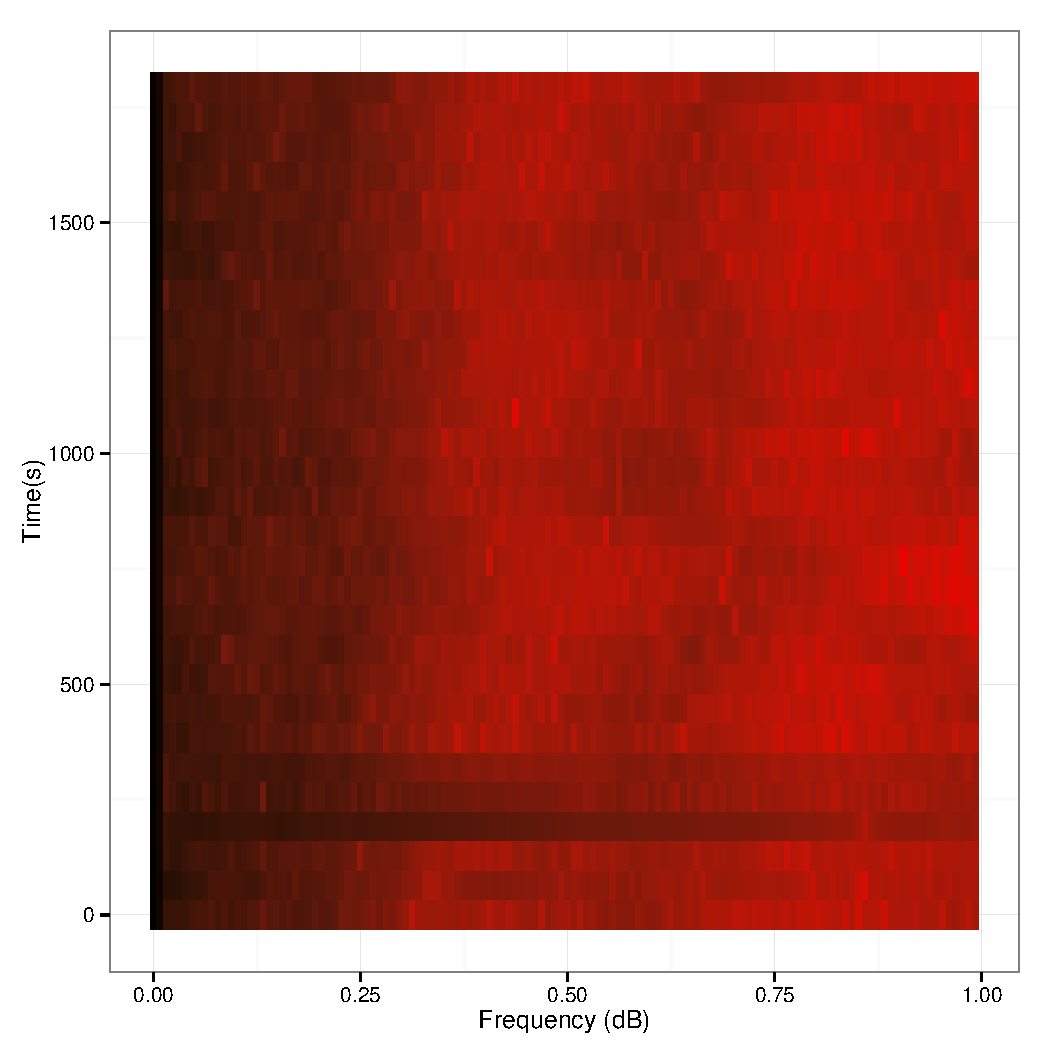
\includegraphics[width=0.8\textwidth]{figure/specGram-1} 

}

\caption[Spectrogram for one example event, each row correspond to a time-point in rr-series while each column correspond to log10(abs(fft)) value of rr-seres at that time-point]{Spectrogram for one example event, each row correspond to a time-point in rr-series while each column correspond to log10(abs(fft)) value of rr-seres at that time-point. The rr-series is divided into 128 equal number of windows with 16 observations overlapping.}\label{fig:specGram}
\end{figure}


\end{knitrout}

For the classification of different activity, I have stacked these frequencies for various Activity for different persons and series, so that each stack refer to some specific combination and the row corresponds to a time scale of some segment of the series and the column corresponds to the frequency of that segment. I have presented the stacking of some of the combination in figure-\ref{fig:SpecGramStack}.

\begin{knitrout}
\definecolor{shadecolor}{rgb}{0.969, 0.969, 0.969}\color{fgcolor}\begin{figure}[H]
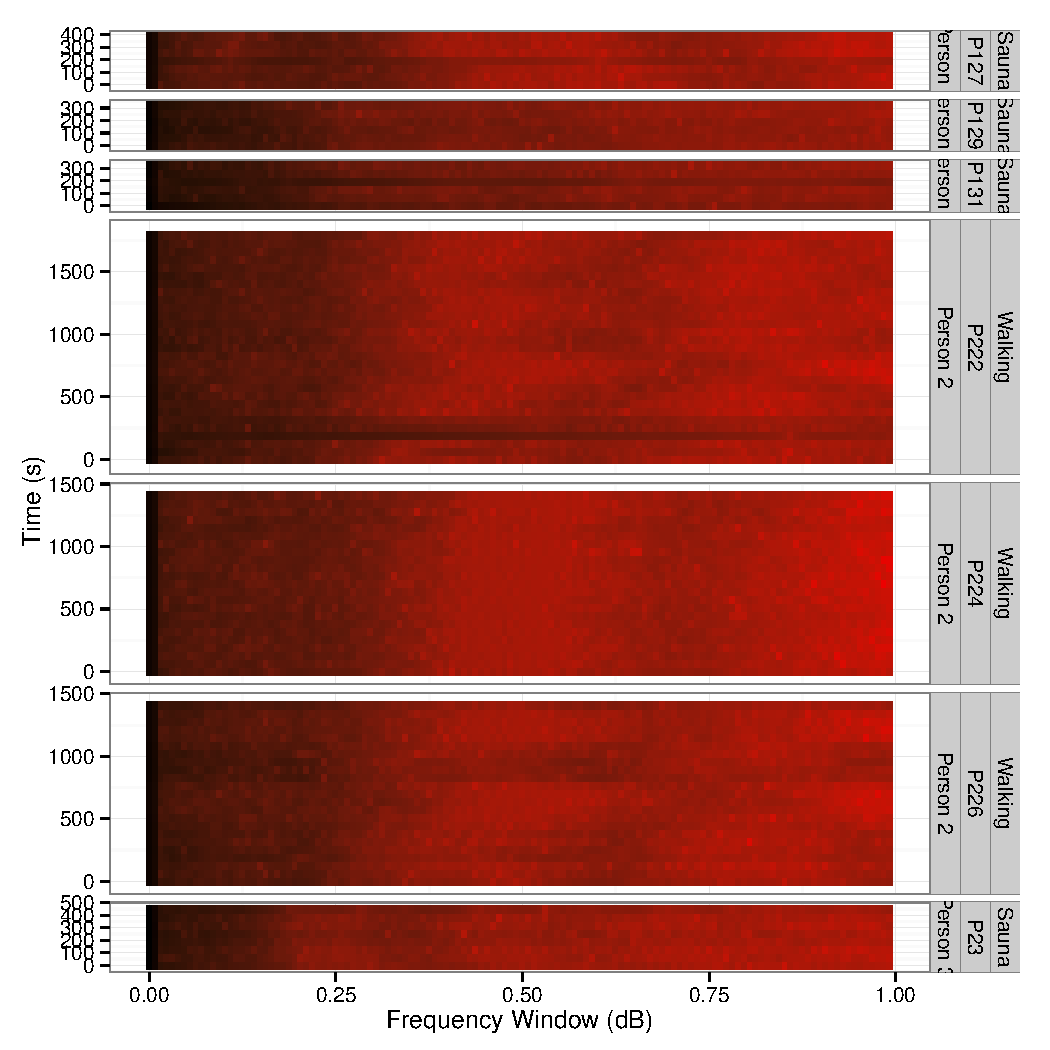
\includegraphics[width=\textwidth,height=0.83\textheight]{figure/SpecGramStack-1} \caption[Stacking of specgram row over row (rbind) with the same frequency window size(128)]{Stacking of specgram row over row (rbind) with the same frequency window size(128)}\label{fig:SpecGramStack}
\end{figure}


\end{knitrout}

If I use this whole matrix for analysis of classification of differnt events, will it be the case of repeated measurement and suffer a problem. I have also tried to take the column mean, i.e. mean over differnt time-points for each frequency column. In that case, I will end up with one row for each of the combination for a person and activity. In that case, I will have very few observation and very poor classification due to the attempts to generalise a lot from the frequencies. Hope to get some suggestion at this last period,

\vspace{2cm}
\noindent Best Regards, \\
Raju Rimal


\end{document}
